%!TEX root = ../report.tex

\clearpage
\chapter{Evaluation}
\label{ch:evaluation}
This chapter presents the evaluation of documented patterns and overall system
against the key drivers of the architecture which already presented in Chapter
\ref{ch:stakeholders}. PBAR\cite{pbar} method is used to carry out the
evaluation. Force Resolution Maps (FRM) are also utilized to present the result.

\begin{table}[H]
\centering
\caption{Force Resolution Maps definition.}
\label{tab:frm-table}
\begin{tabular}{cl}
\textbf{Value} & \textbf{Definition} \\ \toprule
            $-2$   & Big negative impact \\
            $-1$   & Small negative impact \\
            $0$    & Neutral \\
            $+1$   & Small positive impact \\
            $+2$   & High positive impact 
\end{tabular}
\end{table}

\section{Patterns}
\subsection{Client-Server}
\subsection{Layers}
This pattern gives positive implication to portability as clear separation of
containers, Docker daemon, Docker registry, and Docker client makes Docker
portable and loosely coupled. Utilizing Docker registry also promotes sharing
images, which make it easier to deploy an application without knowing what
platform running below it. Exposing TCP/IP connection, specifically REST,
contributes to negative effect on the security. It means that any unwanted
connections or attacks could possible exploit this hole. However, this weak
point is compensated by other patterns. Furthermore, Decoupling some components
means that the components below or above can be replicated in order to gain more
reliability as it has more availability. Thus, this patterns give positive
effect to the reliability. The summary of the Layers pattern evaluation is shown
in FRM in Figure \ref{fig:layers-frm}.

\begin{figure}[H]
\centering
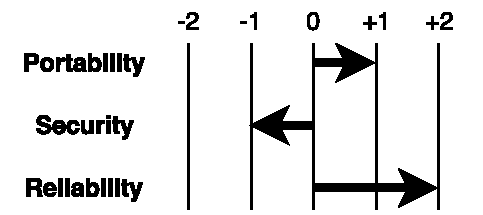
\includegraphics[scale=0.7]{6-evaluation/images/layers_frm.pdf}
\caption{Force Resolution Map for Layers pattern.}
\label{fig:layers-frm}
\end{figure}

\subsection{Shared repository}
\subsection{Event-Driven Messaging}
\subsection{Direct Authentication/Brokered Authentication}
\subsection{Plugin}
\subsection{Proxy}

\section{Overall system}